\section{Introduction}

\subsection[Overview]{History of Cryptocurrency}
\begin{table}
\renewcommand\arraystretch{1.4}\arrayrulecolor{blue}
\captionsetup{singlelinecheck=false, labelfont=sc, labelsep=quad}
\caption{Timeline of Cryptocurrency}%\vskip -1.5ex
\begin{tabular}{@{\,}r <{\hskip 2pt} !{\foo} >{\raggedright\arraybackslash}p{5cm}}
\toprule
\addlinespace[1.5ex]
2009 & Bitcoin\\
1968 & Xerox Palo Alto Research Centre envisage the 'Dynabook\\
1971 & Busicom 'Handy-LE' Calculator\\
1973 & First mobile handset invented by Martin Cooper\\
1978 & Parker Bros. Merlin Computer Toy\\
1981 & Osborne 1 Portable Computer\\
1982 & Grid Compass 1100 Clamshell Laptop\\
1983 & TRS-80 Model 100 Portable PC\\
1984 & Psion Organiser Handheld Computer\\
1991 & Psion Series 3 Minicomputer\\
\end{tabular}
\end{table}

\begin{figure}[ht]
\begin{adjustbox}{center,max width=1.1\textwidth}
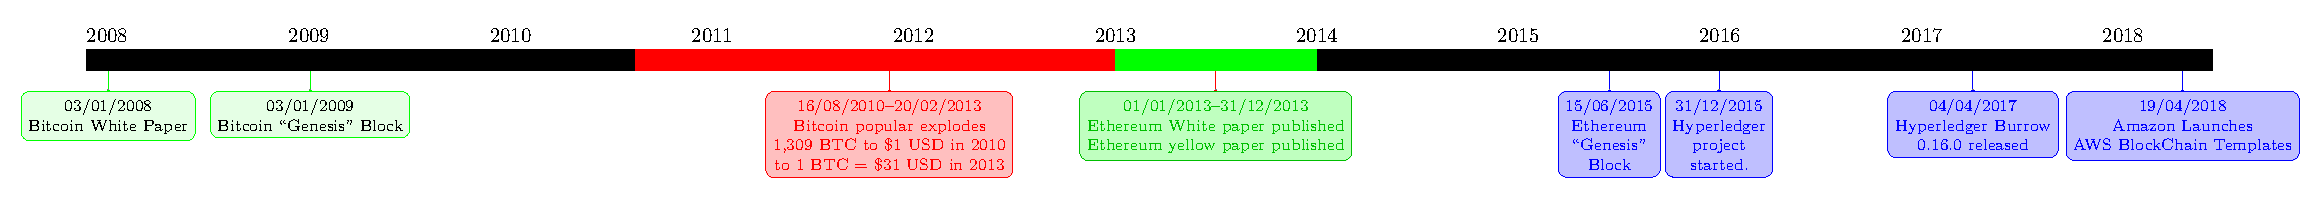
\includegraphics[width=1.2\linewidth]{Diagrams/advancedTimeline.pdf}
\end{adjustbox}
\caption{An example of server-blockchain architecture in a DAPP.}
\label{fig:dappArc}
\end{figure}

In 2008 bitcoin white paper \cite{bitcoinWhitePaper:Online} described a way to solve the double spending problem without a centralized body using blockchain.  Released in July 30, 2015, Ethereum, an open-source platform based on blockchain technology, distinguishes itself from bitcoin through faster transactions, unlimited processing capability for \glspl{smart contract}, and its network is optimized to supports \gls{DApp} \cite{ethereumWhitePaper:Online}.


%%% Contain timeline

\subsection{Decentralized Applications}
%%% ClEAN TIHS UP LATER
	A blockchain is a digitized, decentralized, public ledger of all cryptocurrency transactions. To access websites on the Ethereum blockchain and use dapps a specialized browser is needed, or a plugin like metamask. As shown in 
	Figure \ref{fig:dappArc} dapp \footnotemark, a user's transactions on the application is publicly broadcasting to the blockchain. 
	Implementing architecture for blockchain 
	applications \footnotemark adds an third layer to the standard client-server architecture, however, through the use of interfaces such as the JSON RPC and/or cloud hosting
	 services \footnotemark databases can be query publicly available data on the blockchain. 
	 
\begin{figure}[ht]
\begin{adjustbox}{center,max width=1.1\textwidth}
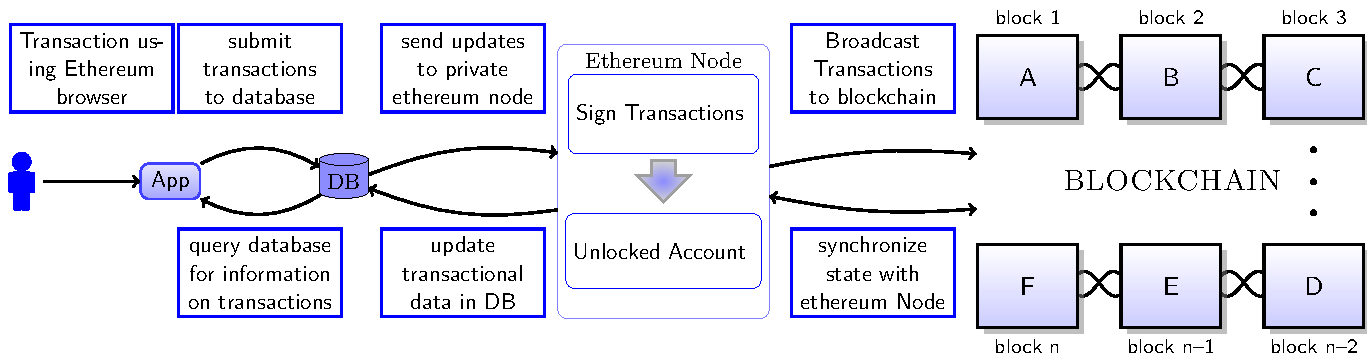
\includegraphics[width=1.2\linewidth]{Diagrams/blockchainInSimpleApp.pdf}
\end{adjustbox}
\caption{An example of server-blockchain architecture in a DAPP.}
\label{fig:dappArc}
\end{figure}

\paragraph{Public and Private Keys}
 \textbf{In a blockchain} system, any key holder can use their private key to sign a piece of data. This results in a signature. In a Dapp, this can be used for:
	Recovering the public key (ethereum account address) of the Author
	Verify if the raw data is the same as the one signed by Author using the public key. 
	Verify whether the message is the same as the one signed by Author
	
	%In order to sign something, a mathematical function is used to "sign" a piece of document/data. A digital signature of a document/data is a number generated using a private key. The private key has a corresponding public key. 
	
	
	
	\begin{figure}[ht]
	\centering
	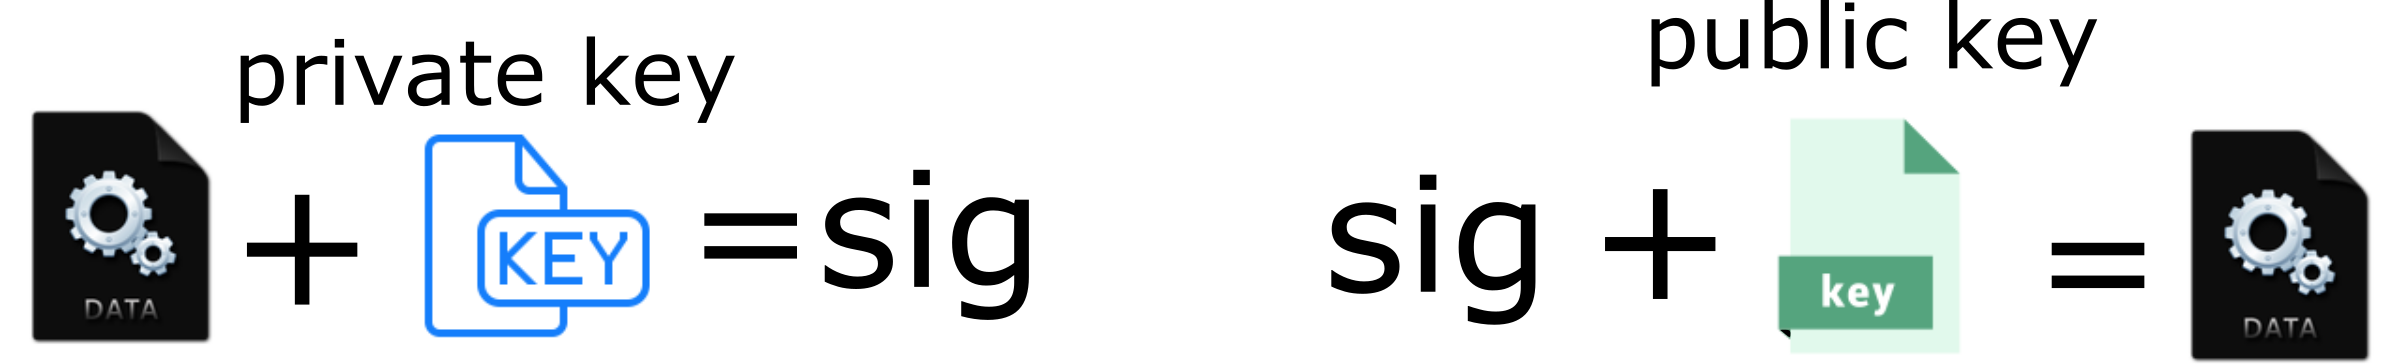
\includegraphics[width=0.5\linewidth]{Diagrams/verifySig.png}
	\caption{Illustrate how public and private keys are used to verify signatures}
	\label{fig:verfSig}
	\end{figure}
	
	\footnotetext[1]{Although, server-blockchain architecture with an abstraction layer resemble traditional applications, other approaches are available such as offline signing with a public node, and client-blockchain in serverless apps \cite{ethereumWhitePaper:Online} and leveraging cloud infrastructure.}
	
	\footnotetext[2]{Amazon recently started offering blockchain on AWS. \cite{ethereumWhitePaper:Online}}
		
	\footnotetext[3]{ \textbf{Signing Transactions}: usning the the ethereum node, use its JSON RPC interface from the application to perform all blockchain operations.}	
	
% refer to medium article, and some other article highlighting the interest in private nodes, https://aws.amazon.com/partners/blockchain/
% https://blog.zeppelin.solutions/designing-the-architecture-for-your-ethereum-application-9cec086f8317
% https://aws.amazon.com/blogs/apn/introducing-aws-blockchain-partners/

%		To access websites on the Ethereum blockchain and use dapps a specialized browser is needed, or a plugin like metamask. 

\subsection{Smart Contracts}